So far the applications of the structures we have discussed are primarily useful at compile- or design-time.
In this section we will discus \acs{TETRiS}, a hybrid mapping approach where the structure of mapping symmetries are useful at run-time.

In Section~\ref{sec:symmetries} we saw how the symmetries of the mapping problem define multiple mappings to be equivalent.
We expect mappings that are equvialent to have the same runtime or energy cosumption. Indeed, the simulation results are identical for equivalent mappings.
When leveraging this structure for \ac{DSE}, we consider only one of the multiple equivalent mappings, disregarding the rest, since they yield identical results in a simulation.
The \acf{TETRiS} approach~\cite{goens_scopes17} leverages this property in a complementary fashion, by selecting equivalent variants at run-time according to the current system load.
While this works for a single mapping, the strength of \ac{TETRiS} lies in selecting from different mappings with different properties first and using the equivalent variants to find a multi-application schedule.

\begin{figure*}[th]
	\centering
	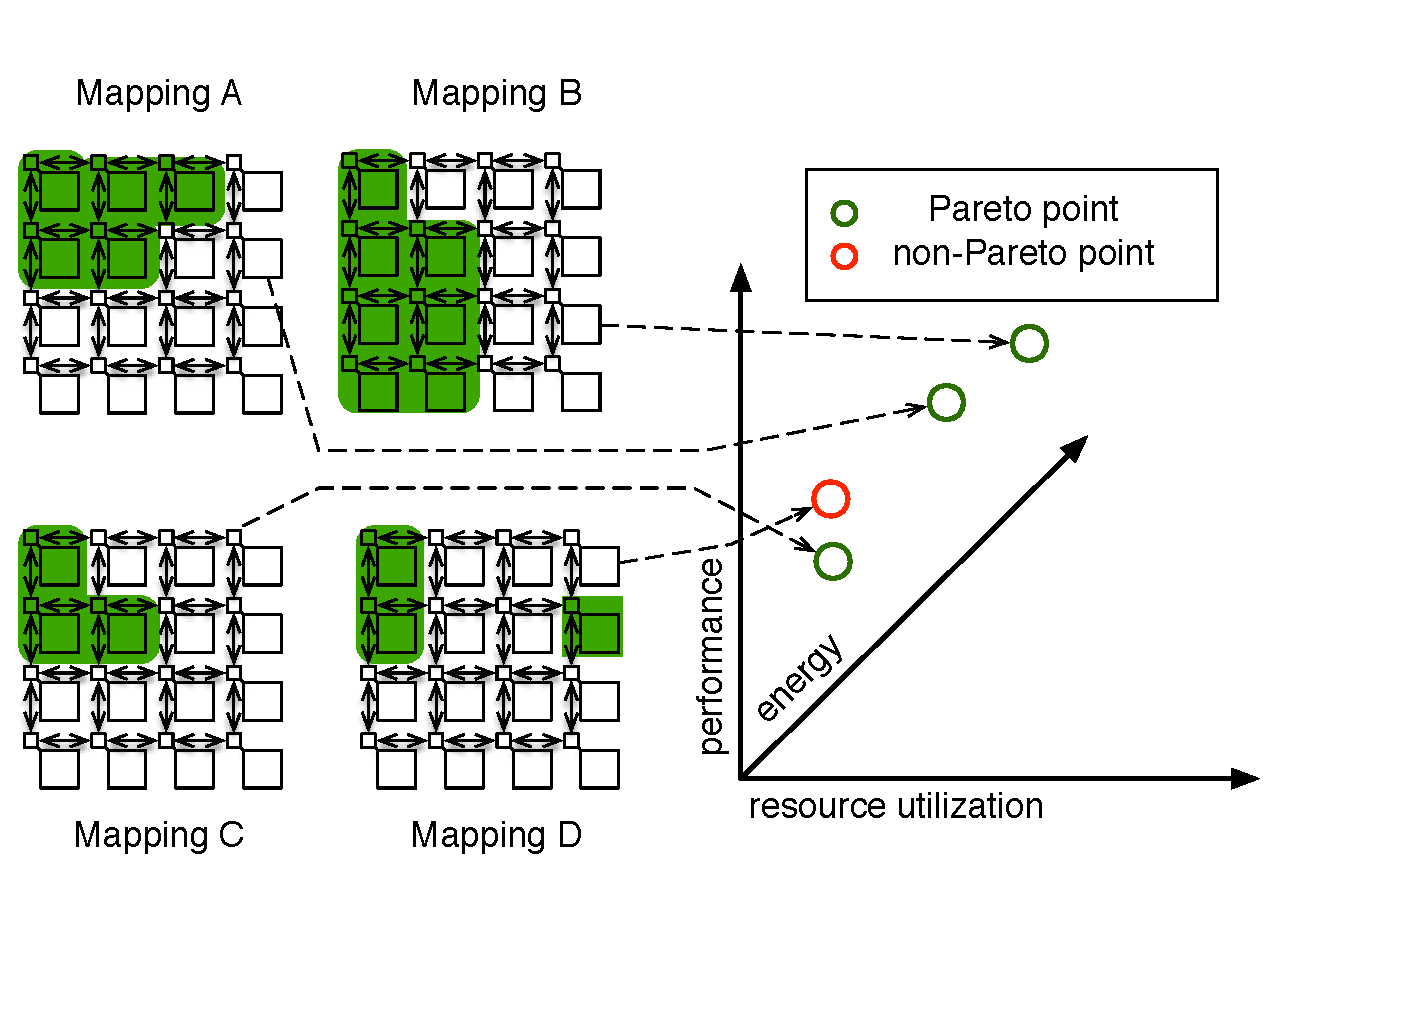
\includegraphics[width=0.7\textwidth]{figures/pareto_mappings.pdf}
	\caption{An illustration of Pareto points in the mapping space.}
	\label{fig:tetris_pareto}
\end{figure*}

The different mappings \ac{TETRiS} chooses from are, ideally, Pareto points in the space of properties we are interested in.
Figure~\ref{fig:tetris_pareto} illustrates this for the properties energy, performance and resource utilization.


The selection algorithms based on the desired properties are beyond the scope of this thesis, but \mocasin has implementations of multiple such algorithms~\cite{khasanov_date20}.
Once a mapping has been selected for each application, they need to be combined in a multi-application mapping.
The ...


\begin{figure*}[th]
	\centering
	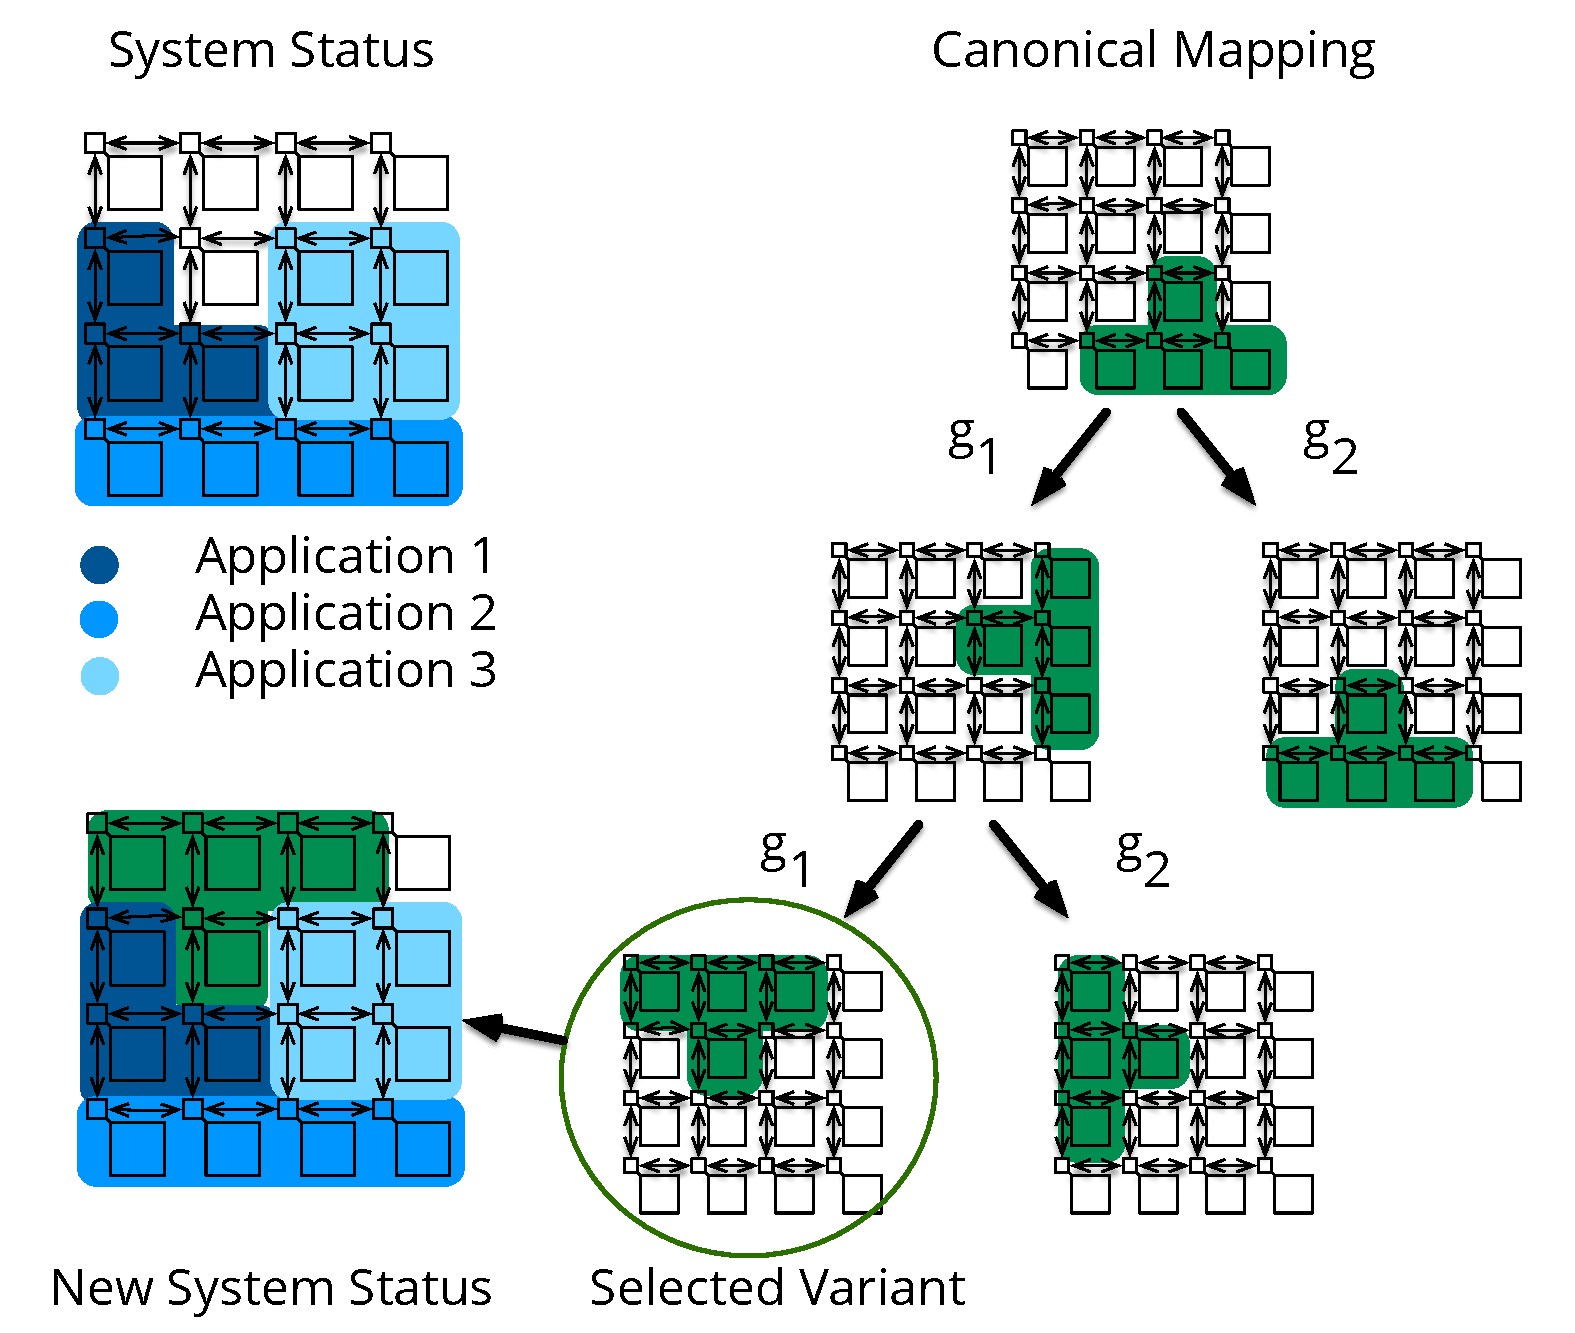
\includegraphics[width=0.8\textwidth]{figures/Variant_Selection.pdf}
	\caption{Variant selection in \ac{TETRiS}.}
	\label{fig:tetris_variant_selection}
\end{figure*}

Figure~\ref{fig:tetris_flow} shows the general flow of the hybrid \ac{TETRiS} approach. 
In a compile-time phase, 

\begin{figure*}[th]
	\centering
	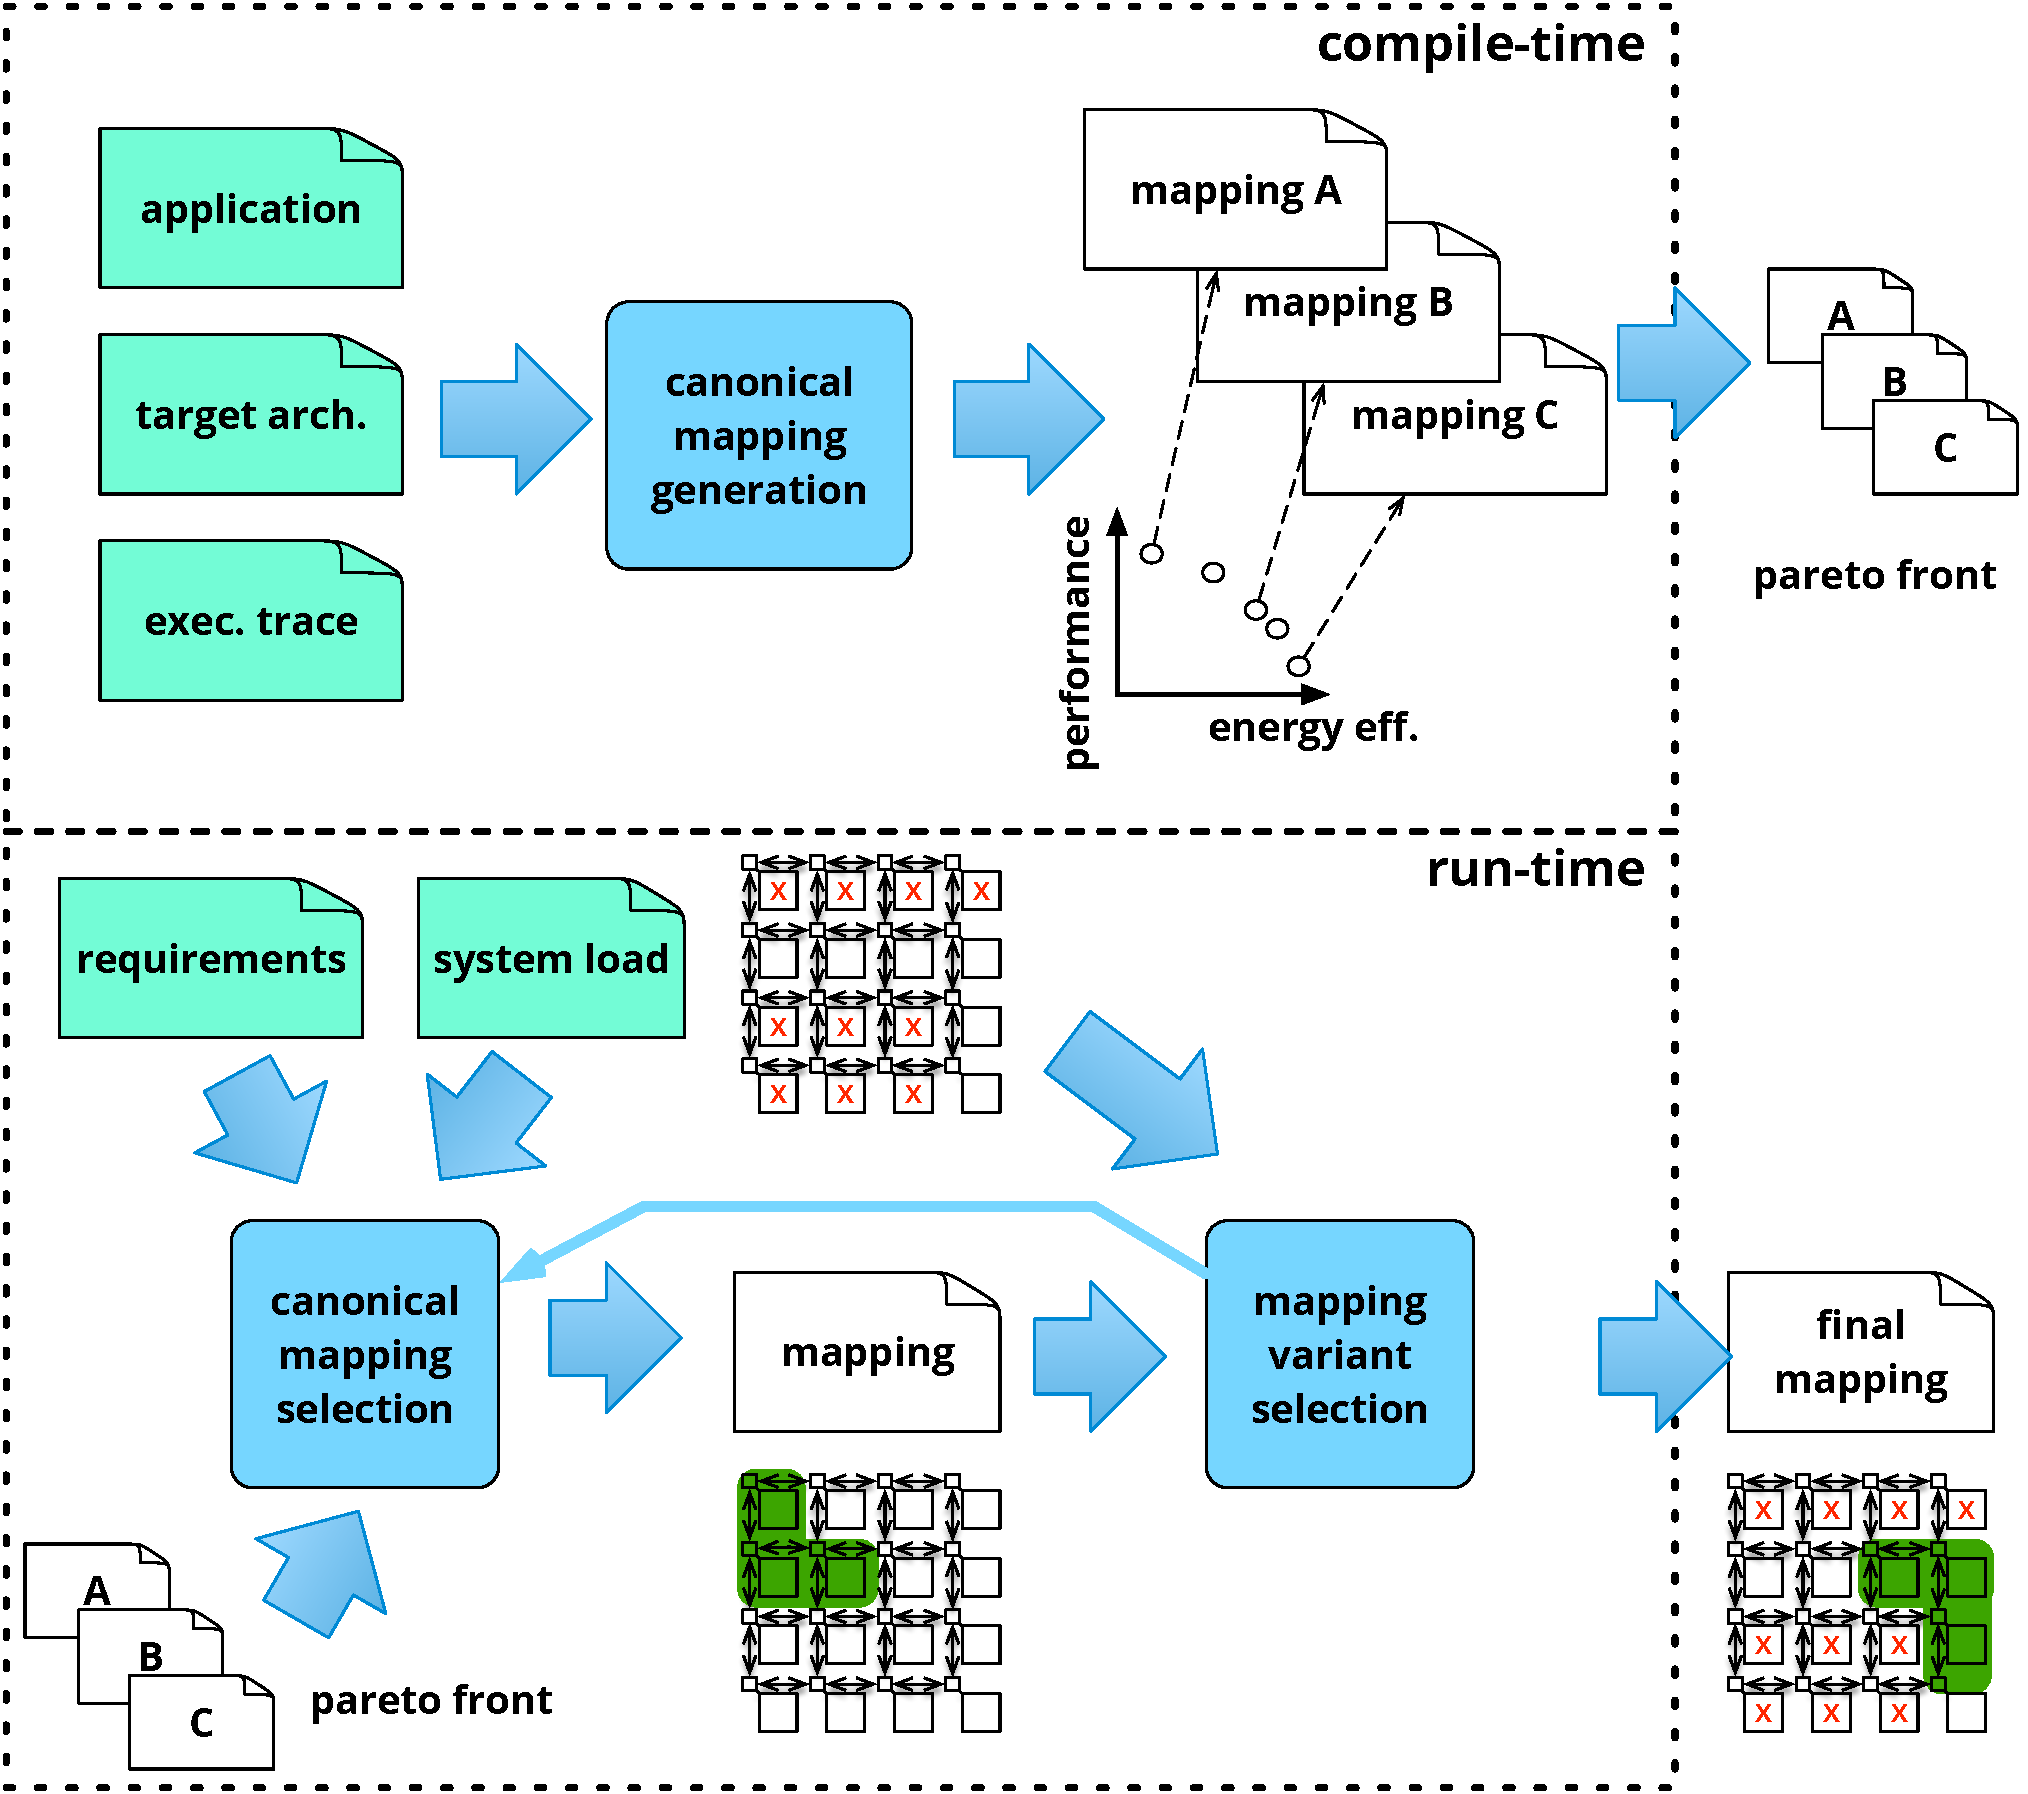
\includegraphics[width=1.00\textwidth]{figures/tetris_flow.pdf}
	\caption{The \ac{TETRiS} flow.}
	\label{fig:tetris_flow}
\end{figure*}


